% !BIB program = bibtex
% !TeX root = ../main.tex

\chapter{Problem Formulation}

In this chapter, we will introduce the scenario of the carpooling fairness problem. Then formulate the problem into a mathematical model with given parameters and decision variables.

\section{Problem Description}

The object of this research is to minimize the maximum percentage of cost saving when a passenger chooses to carpool, with consideration of the number of drivers, car capacity and routing limit constraints.

Take Figure 3-1 as an example scenario; Passenger 1 and Passenger 2 are requesting a trip. When Passenger 1 chooses to take a ride by himself/herself, called "exclusive" riding shown as Figure 3-2, it would cost \$5. We can describe the scenario as a shortest path problem from $S$ to $D_1$, and $P_1$ is a must-pass node. We use Steiner tree to solve this kind of shortest path problem with must-pass nodes. Passenger 2's "exclusive" riding would also cost \$5 in Figure 3-3. In this case, it would be a shortest path problem from $S$ to $D_2$ with $P_2$ as a must-pass node.

When the passengers choose to take a carpool, which is called "sharing" riding. We can describe the scenario as a shortest problem from $S$ to $D_1$ with $P_1$, $P_2$ and $D_2$ as must-pass nodes or $S$ to $D_2$ with $P_1$, $P_2$ and $D_1$ as must-pass nodes. In Figure 3-4 is one of the best case, which would cost \$8 for all the passengers, in Figure 3-5 would cost the same \$8 and both of the fares they could share are \$5 ( $\overline{P_2D_1}$ and $\overline{P_2D_2}$ respectively); however, in Figure 3-4 would cost $\overset{\overline{P_1P_2}}{1} + \frac{1}{2} \times \overset{\overline{P_2D_1}}{5} = \$3.5$ for Passenger 1 and $\frac{1}{2} \times \overset{\overline{P_2D_1}}{5} + \overset{\overline{D_1D_2}}{1} = \$3.5$ for Passenger 2, in Figure 3-5 would cost $\overset{\overline{P_1P_2}}{1} + \frac{1}{2} \times \overset{\overline{P_2D_2}}{5} + \overset{\overline{D_2D_1}}{1} = \$4.5$ for Passenger 1 and $\frac{1}{2} \times \overset{\overline{P_2D_2}}{5} = \$2.5$ for Passenger 2.

\begin{figure}[htp]
  \centering
  \captionsetup{justification=centering}
  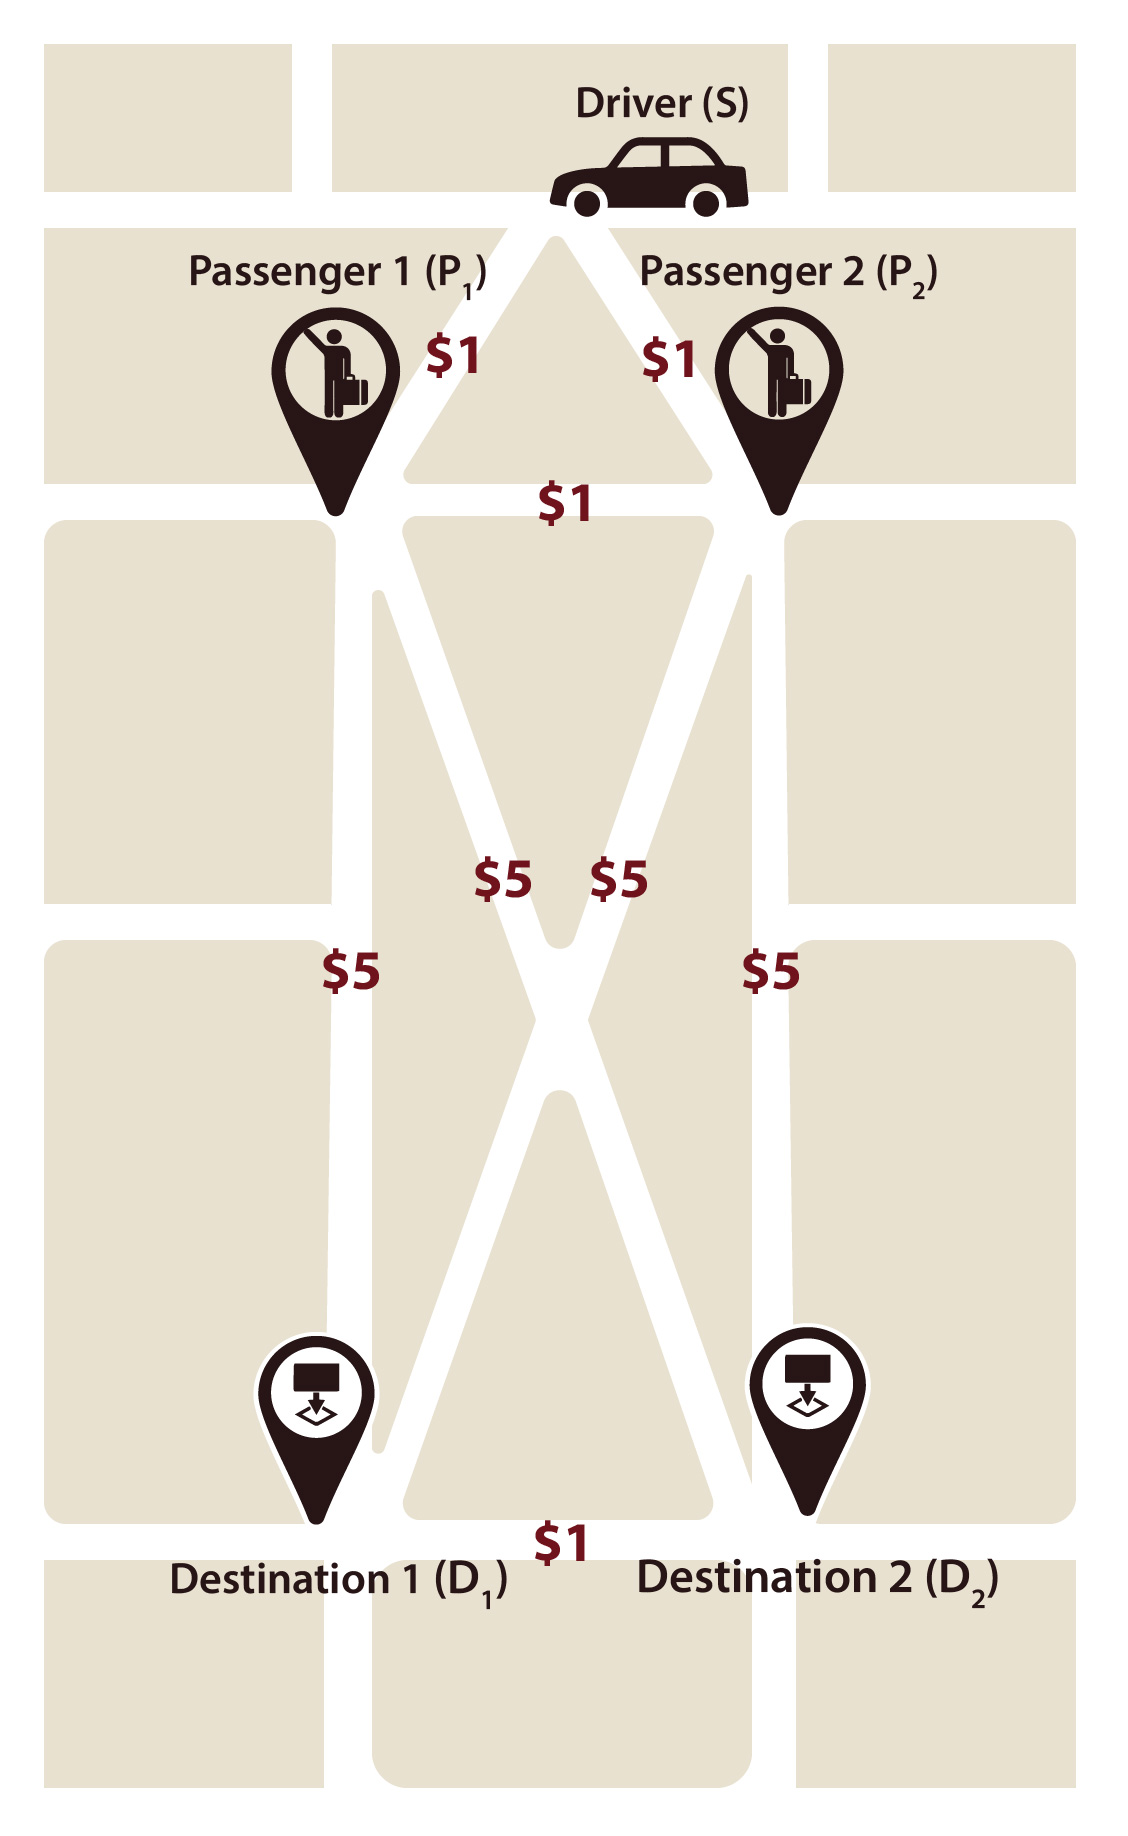
\includegraphics[width=6cm]{figures/mapV2.jpg}
  \caption{Example road network with driving fare and points of passengers and their destinations}
\end{figure}

\begin{figure}[htp]
  \centering
  \captionsetup{justification=centering}
  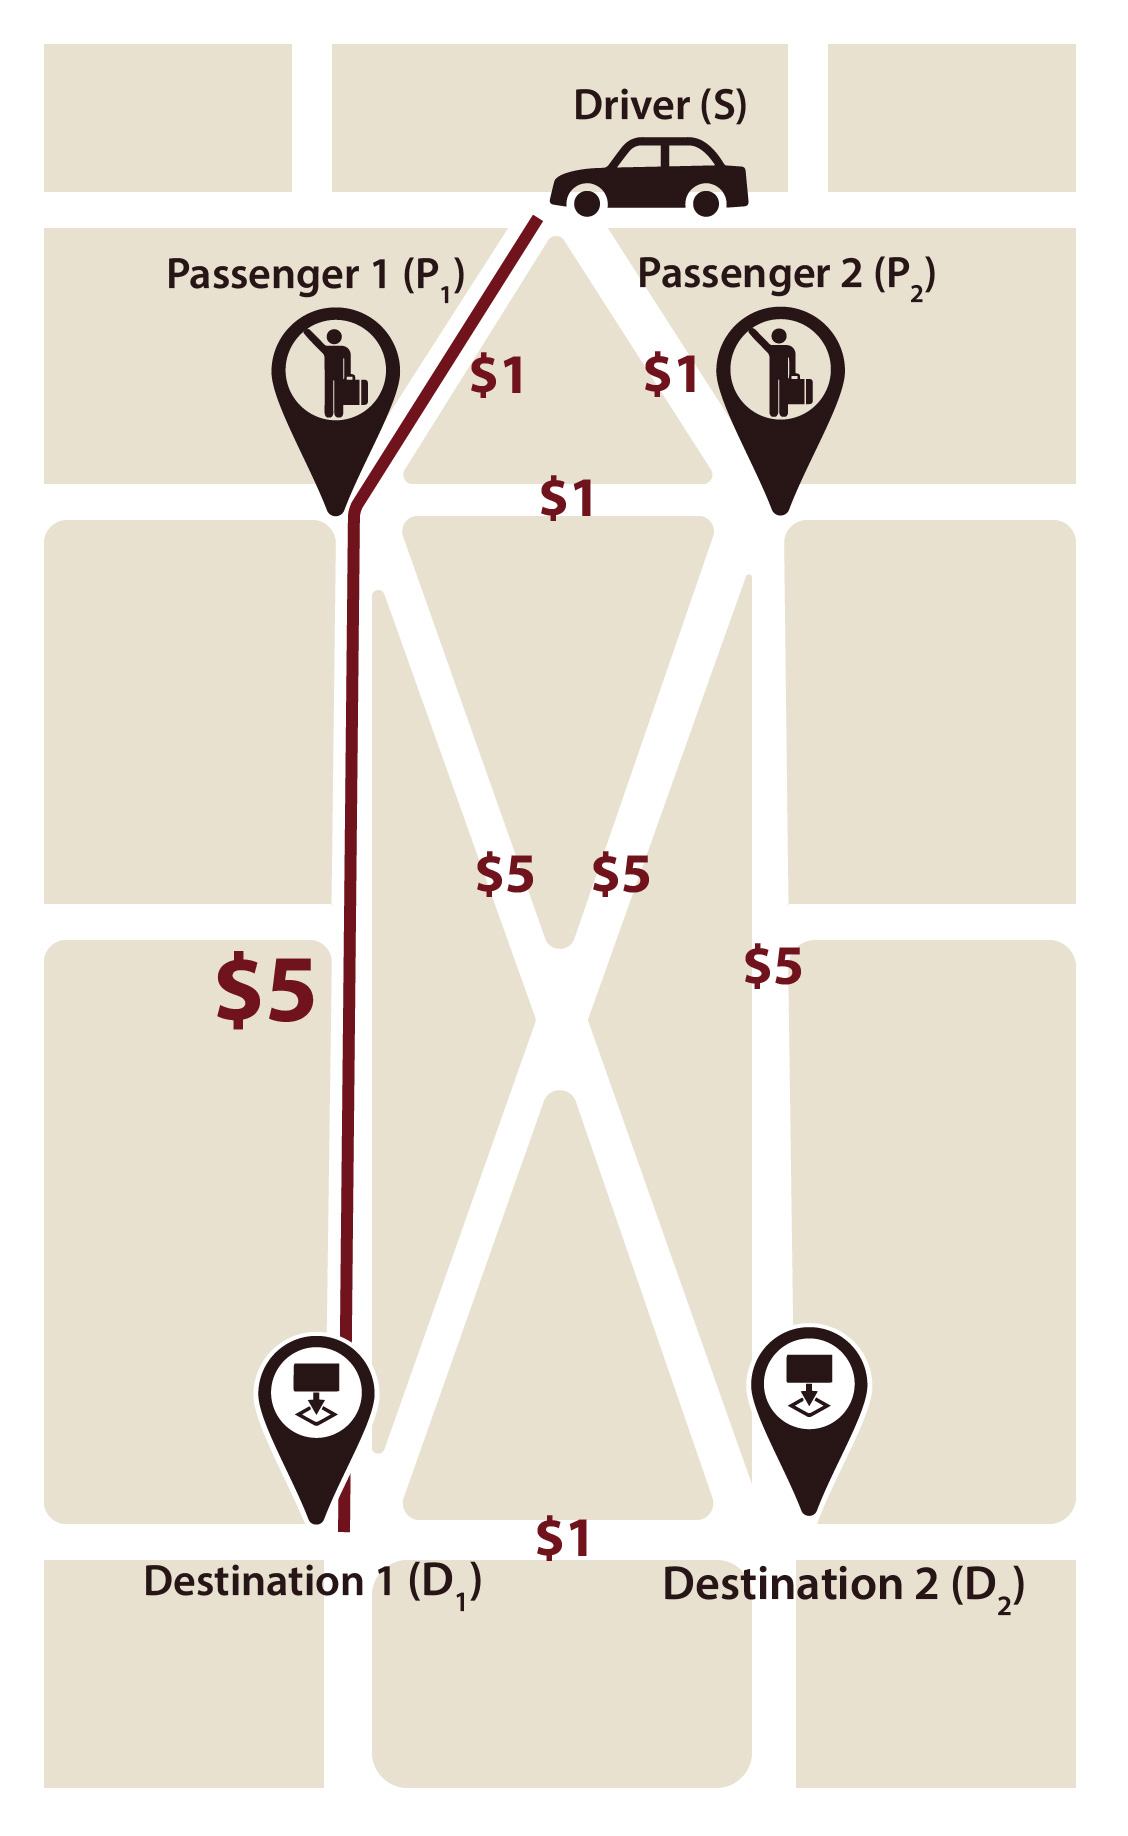
\includegraphics[width=6cm]{figures/mapV2_1.jpg}
  \caption{Best routing path when the driver only serving Passenger 1}
\end{figure}

\begin{figure}[htp]
  \centering
  \captionsetup{justification=centering}
  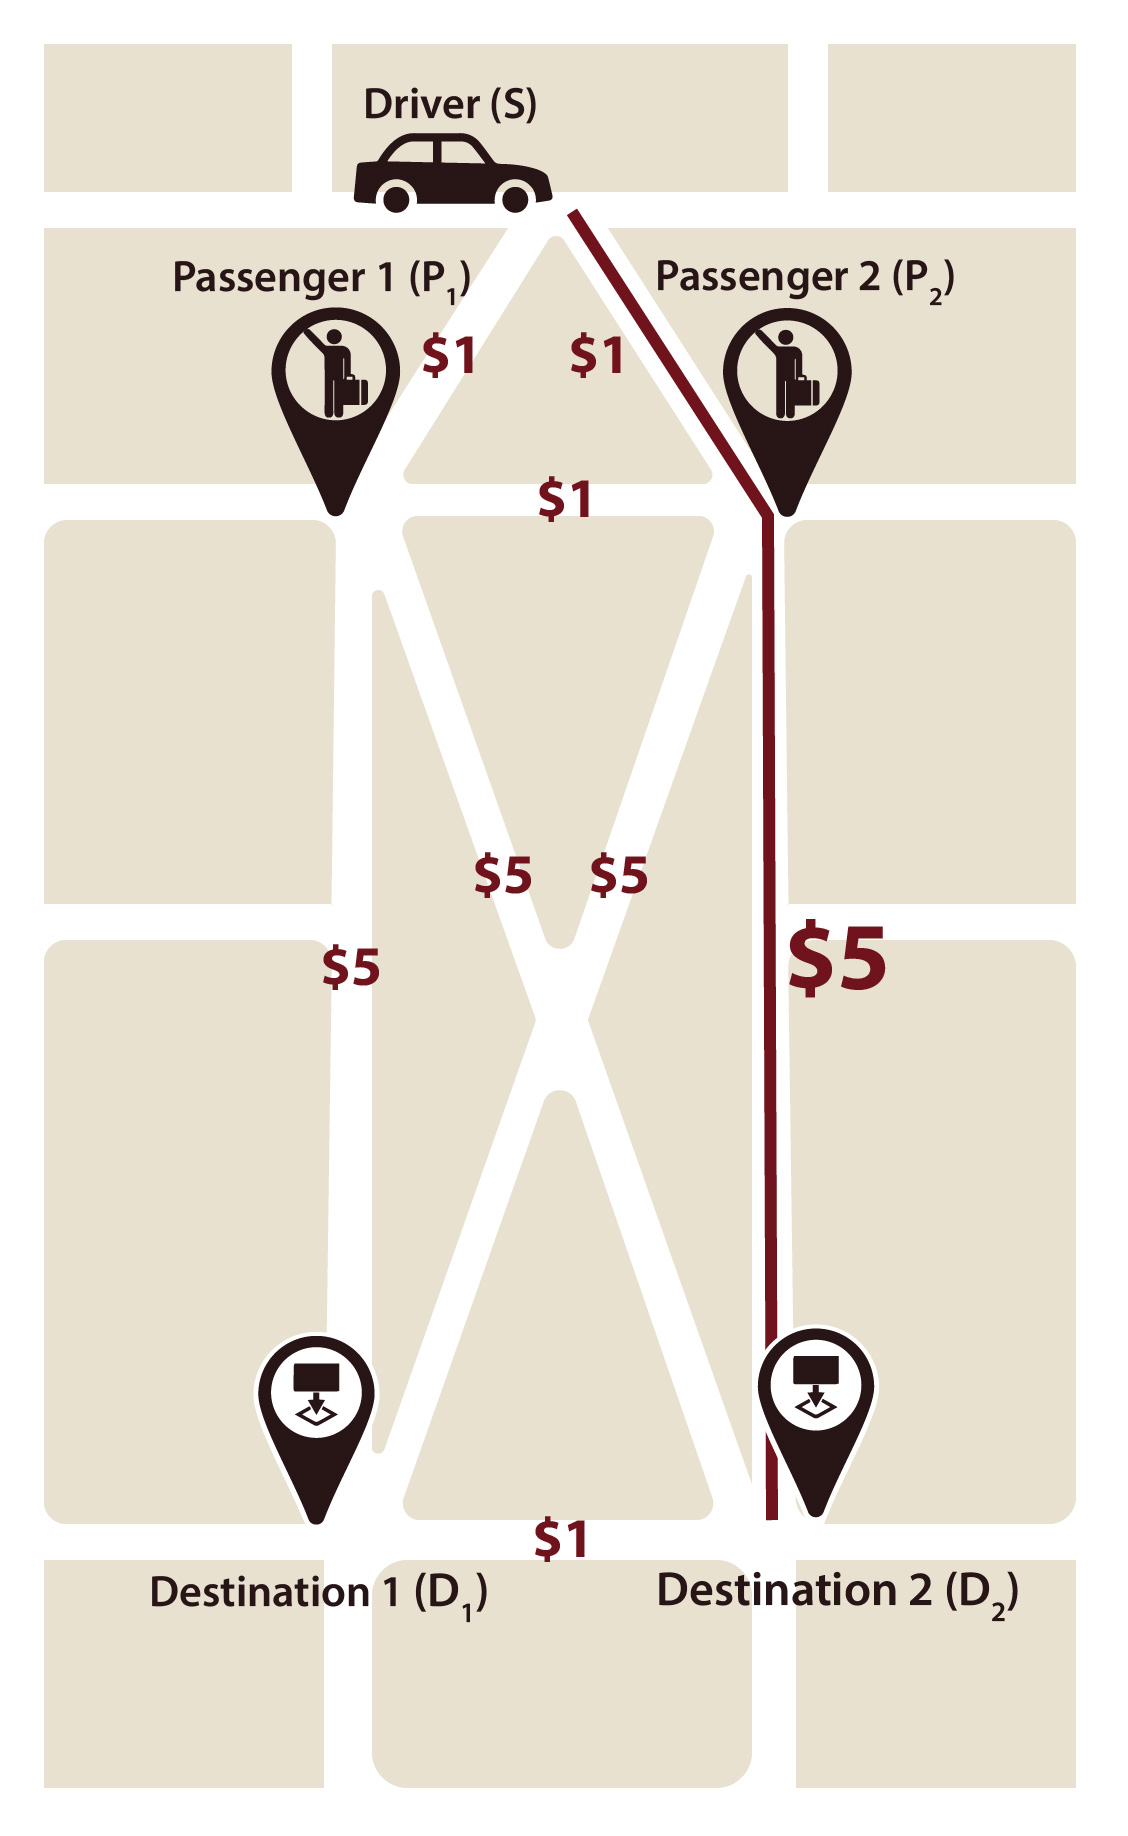
\includegraphics[width=6cm]{figures/mapV2_4.jpg}
  \caption{Best routing path when the driver only serving Passenger 2}
\end{figure}

\begin{figure}[htp]
  \centering
  \captionsetup{justification=centering}
  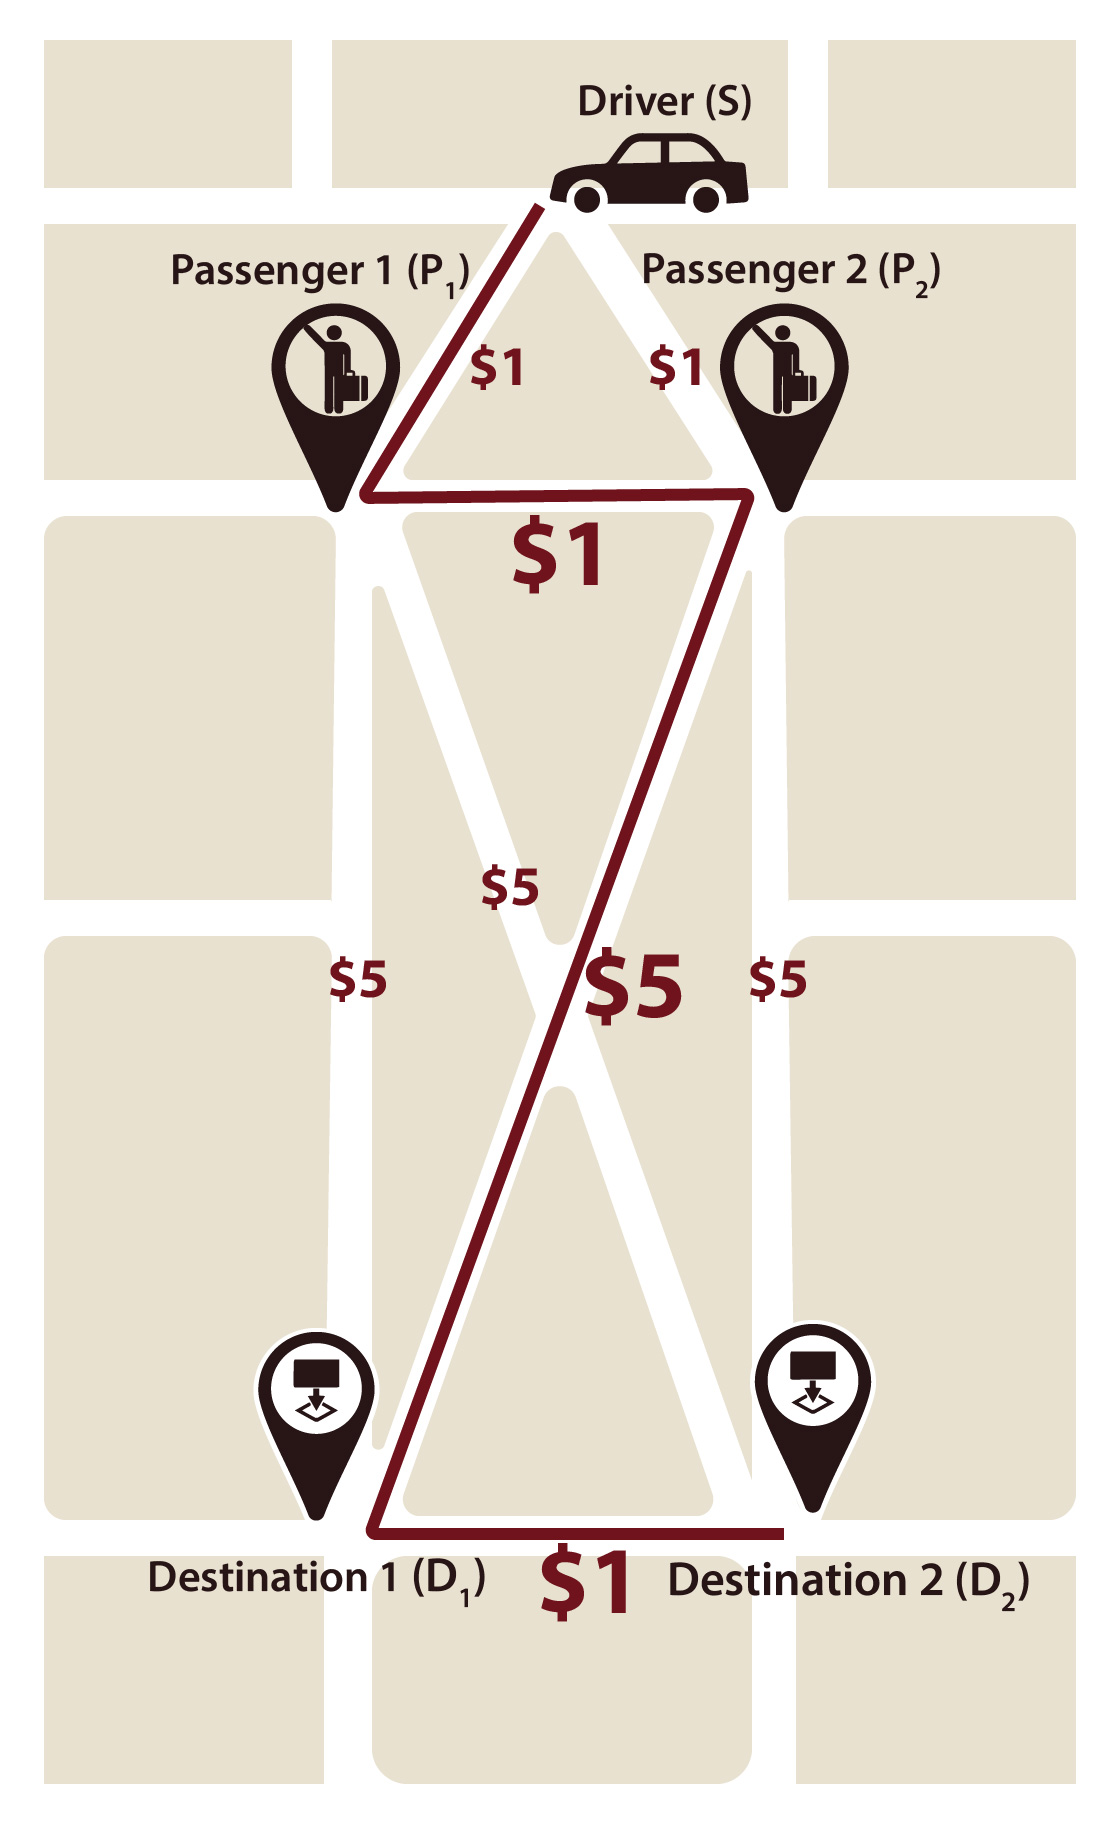
\includegraphics[width=6cm]{figures/mapV2_2.jpg}
  \caption{One of the best routing when both Passenger 1 and Passenger 2 carpool}
\end{figure}

\begin{figure}[htp]
  \centering
  \captionsetup{justification=centering}
  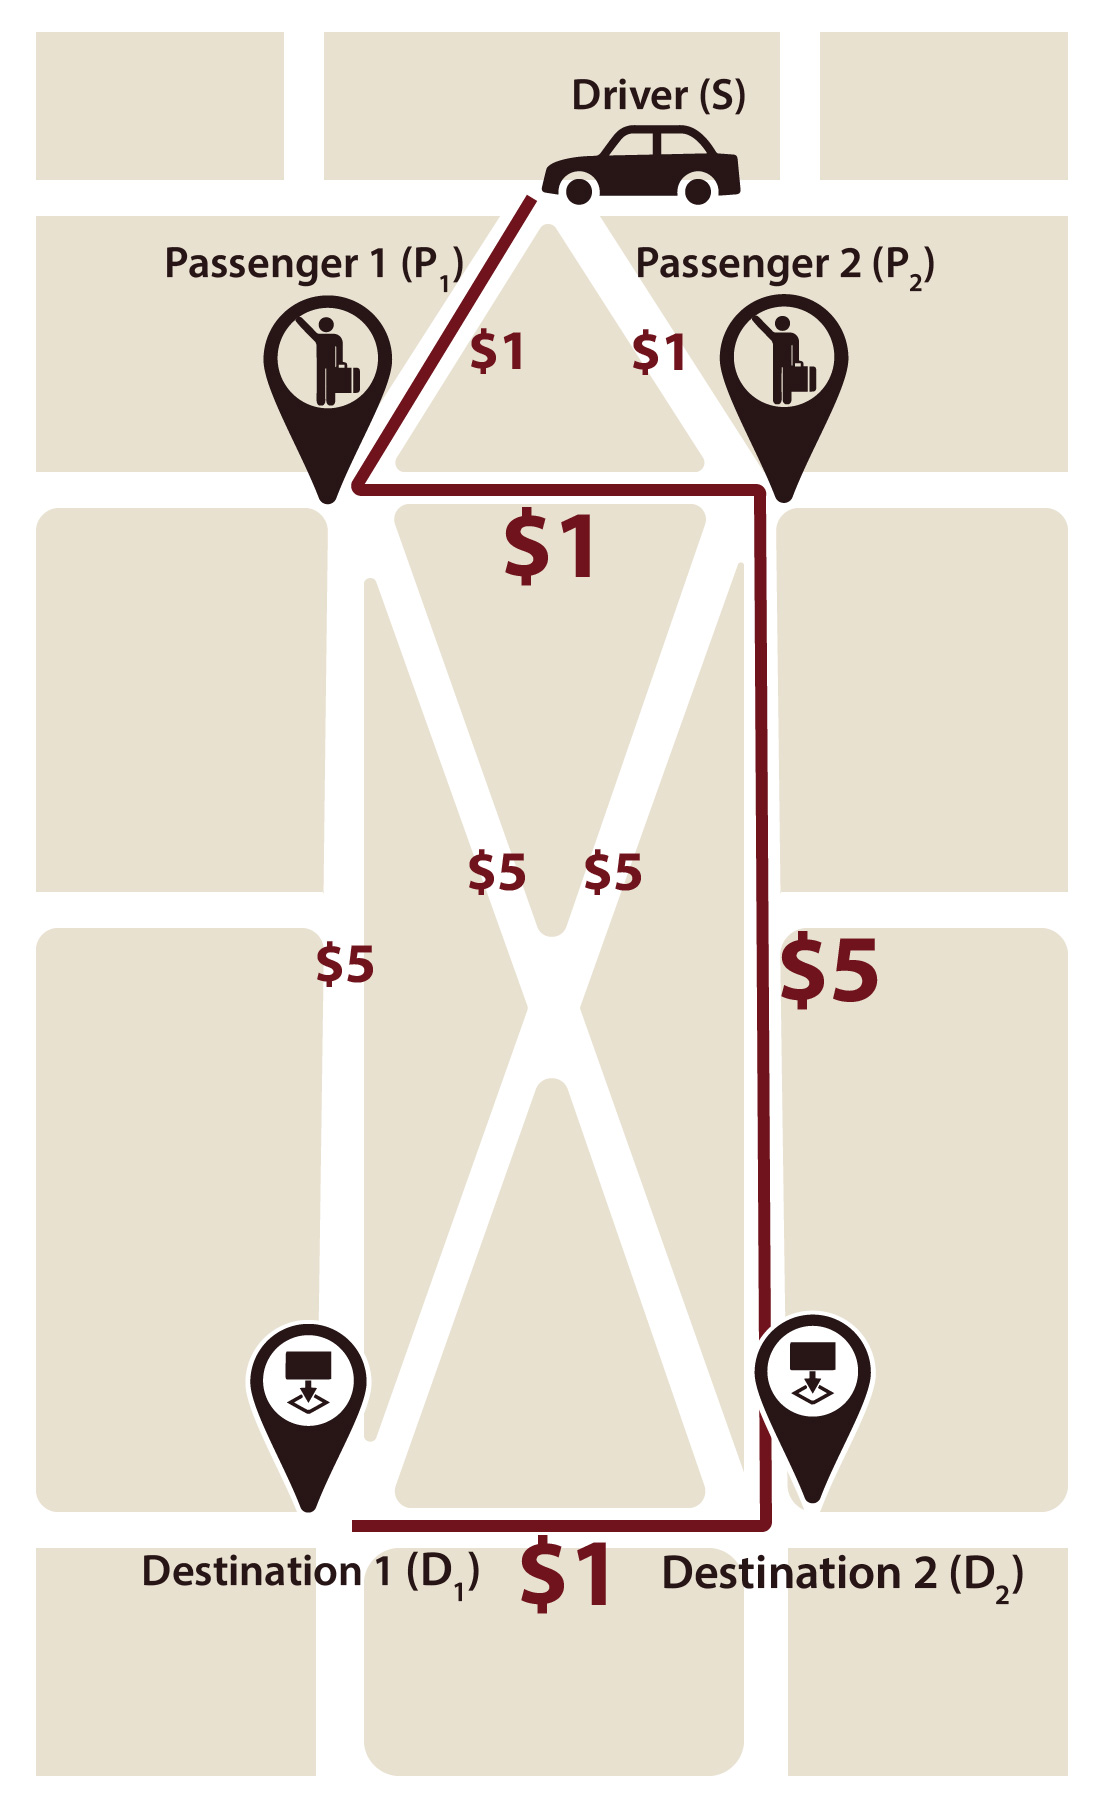
\includegraphics[width=6cm]{figures/mapV2_3.jpg}
  \caption{Another best routing when both Passenger 1 and Passenger 2 carpool}
\end{figure}
\newpage

\subsection{Assumptions}

There are three assumption in out system:

\begin{enumerate}
  \item Every driving request only includes one passenger. This driving request will be split into multiple one-person driving request for a driving request with multiple people.
  \item System calculation time is not considered, that is, assume that drivers' location will still keep unchanged after the time of system calculation.
  \item The carpooling fare is shared equally by the time passengers in the vehicle. For a specific link in the route with $n$ passengers, the fare of the link for a passenger will be divided by $n$.
 \end{enumerate}

\subsection{Fairness of Vehicle Dispatching}

In order to consider the fairness when dispatching driver, we introduce Jain's fairness index to avoid unfair situation:

$Firness\ Index = f_A(x) = \frac{\left(\sum\limits_{i=1}^{n} x_i\right)^2}{n \sum\limits_{i=1}^{n} x_i^2}$

We take accumulate driving requests that a driver has received as the metrics for fairness. That is, when a driver receives more driving requests in the past, he/she should give his/her chance of receiving a new driving request to the one who takes fewer driving requests.

As a new driving request comes, we need to ensure our system must get more or at least keep the same fairness. Hence, we form a constraint that the fairness index can not decrease compared to the previous fairness index.

However, when the driving resource changes, such as a new driver joins our system, it will violate our constraint for fairness. Because the newcomer has not taken any driving request before, the fairness will decrease. Even if a driver leaves our system, the fairness will increase or decrease due to the driver's situation. As a result, we need to reset the fairness index to the initial state and reset all the drivers' accumulated driving requests to 0. Nevertheless, it will make the fairness index's denominator to 0, which can not be divided. To avoid this situation, we assign a virtual driver with one accumulated driving request, which will make the fairness index to $\frac{1}{(n+1)}$, where $n$ is the number of drivers in our system. Moreover, for any situation that the fairness index will decrease when dispatching a new driving request, the fairness will reset.

\newpage

\section{Mathematical Model}

We will go through the detailed given parameters and decision variables in the mathematical model before describing our mathematical model.

\renewcommand\arraystretch{1.5}
\par
\begin{table}[ht]
  \centering
  \caption{Notations of given parameters}
  \begin{tabularx}{\textwidth}{cX}
  \toprule
  Notation & Description \\
  \midrule
    $B_r$ & Set of passengers that driver $r$ has picked up, where $r \in R$ \\
    $D$ & Set of destinations in the system (take $k$ as index) \\
    $L$ & Set of links on the road network \\
    $L_c$ & Set of links on the road network that pass by the passenger $c \in C$ \\
    $L_d$ & Set of links on the road network that pass by the destination $d \in D$ \\
    $C$ & Set of passengers in the system (take $j$ as index) \\
    $P_r$ & Set of all paths for driver $r$, where $r \in R$ \\
    $P_{rw}$ & Set of all paths for driver $r$ from initial location to a passenger or a destination, where $r \in R$ and $w \in W$ \\
    $P_{rc_i}$ & Set of all paths for driver $r$ from initial location to passenger $c_i$, where $r \in R$ and $c_i \in C$ \\
    $P_{rd_i}$ & Set of all paths for driver $r$ from initial location to destination $d_i$, where $r \in R$ and $d_i \in D$ \\
    $Q_r$ & Maximum load capacity for driver $r$, where $r \in R$ \\
    $R$ & Set of drivers in the system (take $i$ as index) \\
    $W$ & Set of passengers or destinations in the system, where $W = P \cup D$ \\
    $f_l$ & The fare for the link $l$, where $l \in L$ \\
    $g_r$ & The capacity that the driver $r \in R$ has loaded in the previous decision round. \\
    $\alpha$ & The fairness index in the previous decision round. \\
    $\delta_{pl}$ & Indicator function which is 1 if link $l \in L$ on the route $p \in P_r$ is selected when driver $r \in R$ goes carpooling; 0 otherwise \\
    $\zeta_{pl}$ & Indicator function which is 1 if link $l \in L$ on the route $p \in P_{rd_i}, i \in \{1,2,3,...,n\}$ is selected when passenger $c_i \in C$ with index $i$; 0 otherwise \\
  \bottomrule
  \end{tabularx}
\end{table}  
\par

\begin{table}[ht]
  \centering
  \caption{Notations of decision variables}
  \begin{tabularx}{\textwidth}{cX}
  \toprule
  Notation & Description \\
  \midrule
    $u_l$ & Binary variable, 1 if link $l \in L$ is on the shortest path; 0 otherwise. \\
    $v_{wp}$ & Binary variable, 1 if route $p \in P_r$ is chosen; 0 otherwise. \\
    $x_p$ & Binary variable, 1 if route $p \in P_r$ is chosen when driver $r \in R$ goes carpooling; 0 otherwise. \\
    $y_p$ & Binary variable, 1 if route $p \in P_{rd_i}, i \in \{1,2,3,...n\}$ is chosen when passenger $c_i \in C$ with index $i$ does not take a carpooling; 0 otherwise. \\
    $z_p$ & Binary variable, 1 if route $p \in P_{rw}$ is chosen; 0 otherwise. \\
    $a_r$ & Total fare that the driver $r \in R$ has earned before current decision round. \\
    $b_r$ & Total fare that the driver $r \in R$ has earned after current decision round. \\
  \bottomrule
  \end{tabularx}
\end{table}  
\newpage

\subsubsection*{Objective Function}

The objective function is to maximize the minimum discount percentage when applying carpooling among passengers in one trip.

\begin{align*}
  max\ min\ \frac{Z_i - carpool\ cost_i}{Z_i} \tag{IP1} \\
  where\ Z_i = \sum_{p \in P_{rd_i}} \sum_{l \in L} y_p \zeta_{pl} a_l \\
\end{align*}

\subsubsection*{Constraints}

\begin{align*}
  \intertext{Constraint 3.1 ensures there is only one path selected for a driver.}
  & \sum\limits_{p \in P_r} x_p \leq 1 \tag{3.1} \\
  \intertext{Constraint 3.2 ensures the selected link on the route we chose is on the shortest path.}
  & \sum\limits_{p \in P_r} x_p \delta_{pl} \leq u_l && \forall l \in L \tag{3.2} \\
  \intertext{Constraint 3.3 ensures all the links pass by the node of passenger or destination we chose is the shortest path.}
  & u_l \leq 1 && \forall l \in L_c \cup L_d \tag{3.3} \\
  \intertext{Constraint 3.4 ensures that all the routes to passengers or destinations we chose is on the shortest path and overlap the route we chose.}
  & \sum\limits_{p \in P_w} z_p \delta_{pl} \leq u_l && \forall w \in W \tag{3.4} \\
  \intertext{Constraint 3.5 ensures the route we chose will only pass by the node of passenger or destination once.}
  & \sum\limits_{p \in P_w} z_p \leq 1 && \forall w \in W \tag{3.5} \\
  \intertext{Constraint 3.6 ensures that we must pick up the passenger before we drop off the passenger.}
  & \sum\limits_{l \in L} \sum\limits_{p \in P_{rc_i}} z_p \delta_{pl} f_l \leq \sum\limits_{l \in L} \sum\limits_{p \in P_{rd_i}} z_p \delta_{pl} f_l && \forall i \in \{1,2,,...,n\}, r \in D \tag{3.6} \\
  \intertext{Constraint 3.7 ensures the fairness index after current decision round will not less than the previous decision round.}
  & \frac{\left(\sum\limits_{r \in R} b_r\right)^2}{\sum\limits_{r \in R} 1 \sum\limits_{r \in R} b_r^2} \geq \alpha \tag{3.7} \\
  \intertext{Constraint 3.8 is the fairness index in the previous decision round.}
  & \frac{\left(\sum\limits_{r \in R} a_r\right)^2}{\sum\limits_{r \in R} 1 \sum\limits_{r \in R} a_r^2} \leq \alpha \tag{3.8} \\
\end{align*}